\documentclass{article}

\usepackage[utf8]{inputenc}
\usepackage{enumitem}
\usepackage{latexsym}
\usepackage{amsfonts}
\usepackage{amsmath,amssymb,amsthm}
\usepackage{amsfonts}
\usepackage{parskip}
\usepackage{listings}

\usepackage{tikz}
\usetikzlibrary{arrows, automata, bending, positioning}

\newcommand{\set}[1]{\{#1\}}
\renewcommand{\epsilon}{\varepsilon}

\title{Homework N}
\author{Asier Garcia Ruiz}

\begin{document}
\maketitle

\newenvironment{question}[2]
{
    {\large \textbf{Question #1.}}\\
    #2\\\\
    \textbf{Answer:}
}{\newpage}

\begin{question}{0}
    {
        I commit to uphold the ideals of honor and integrity by refusing to betray the trust bestowed upon me as a member of the Georgia Tech community.
    }
    Signature: Asier Garcia Ruiz
\end{question}

\begin{question}
    {1a}
    {
        (2 points) Consider the following invalid proof that $A \cup \{\epsilon\}$ is regular if $A$ is regular:

        ``Since $A$ is regular, it has a NFA $N$. We can create an NFA $N'$ for $A \cup \{\epsilon\}$, modifying $N$ by setting the start state to be accepting. Then $N'$ accepts $A \cup \{\epsilon\}$, Q.E.D."

        Show that this proof is invalid by giving a regular language $A$ and an NFA $N$ for $A$, such that constructing $N'$ as described in the ``proof" does not accept $A \cup \{\epsilon\}$.
    }
    Consider the language $A = 1(1)^*0$ i.e. all binary strings starting with some
    number of ones and ending in 0. The NFA for this language is

    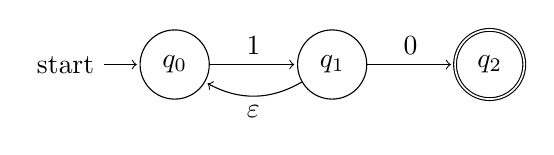
\begin{tikzpicture}[shorten >=1pt,node distance=2cm,on grid,auto]
        \node[state, initial]   (q0)                       {$q_0$};
        \node[state]   (q1)    [right of=q0]                {$q_1$};
        \node[state, accepting]   (q2)  [right of=q1]       {$q_2$};

        \path[->]   (q0) edge node {1} (q1)
        (q1) edge node {0} (q2)
        (q1) edge [bend left] node {$\varepsilon$} (q0)
        ;
    \end{tikzpicture}

    Now if we construct $N'$ as in the proof we get

    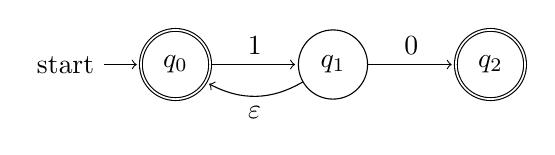
\begin{tikzpicture}[shorten >=1pt,node distance=2cm,on grid,auto]
        \node[state, initial, accepting]   (q0)                       {$q_0$};
        \node[state]   (q1)    [right of=q0]                {$q_1$};
        \node[state, accepting]   (q2)  [right of=q1]       {$q_2$};

        \path[->]   (q0) edge node {1} (q1)
        (q1) edge node {0} (q2)
        (q1) edge [bend left] node {$\varepsilon$} (q0)
        ;
    \end{tikzpicture}

    This implies that $N'$ accepts $(1)^*$, which is not in the language of $A$.
    Therefore, this proof is wrong.
\end{question}

\begin{question}
    {1b}
    {
        (2 points) Suppose you are trying to prove that $L = \{ww\ |\ w \in \Sigma^*\}$ is not regular using the pumping lemma. You have already assumed that $L$ is regular, and let $p$ be the pumping length. Which of the following can you choose as the string $s$ which is pumped and leads to a contradiction? (Circle all that apply.)

        $0^p0^p \qquad 0^p1^p \qquad (01)^p \qquad 0^{p-1}10^{p-1}1$
    }
    $0^{p-1}10^{p-1}1$
\end{question}

\begin{question}
    {1c}
    {
        Give three \textit{different} non-regular languages $A,B,C$ such that the union of the three languages is regular.
    }
    Let $i,j \geq 0$. Consider the three non-regular languages
    \begin{align*}
        L_1 & = \set{0^i1^j : i > j}, \\
        L_2 & = \set{0^i1^j : i < j}, \\
        L_3 & = \set{0^i1^j : i = j}
    \end{align*}

    Then we have that
    \begin{equation*}
        L_1 \cup L_2 \cup L_3 = \set{0^i1^j : i, j \geq 0}.
    \end{equation*}
    Which is regular.
\end{question}

\begin{question}
    {2}
    {
        Let $L^R = \{ w^R | w \in L\}$, i.e. the set of strings which are the reverse of some string in $L$. Show that if $L$ is a regular language, then $L^R$ is also regular.
    }
    If $L$ is regular, we know there is some NFA $N = (Q, \Sigma, \delta, q_0, F)$
    that recognises $L$. Now, we will construct an NFA $N' = (Q', \Sigma', \delta' q_0', F')$
    that recognises $L^R$. We will define the components of $N'$ as follows:
    \begin{align*}
        Q'                      & = Q \cup \set{q_0'},                                  \\
        \Sigma'                 & = \Sigma,                                             \\
        q_0'                    & = q_0' \quad \text{i.e. a new state},                 \\
        F'                      & = \set{q_0} \quad \text{i.e. the start state of $N$}.
        \intertext{Now, we will define $\delta'$ as follows, for all $q_i, q_j \in Q, a \in \Sigma$}
        \delta'(q_i, a)         & = q_j \quad \text{if } \delta(q_j, a) = q_i
        \intertext{Finally, for all $q \in F$ we define}
        \delta'(q_0', \epsilon) & = q.
    \end{align*}

    In summary, we create a new start state and draw $\epsilon$-transitions from the
    new start to every accepting state in $N$. Then, we reverse all the original
    transitions, and set the new accepting state to the start state of $N$.
    This new NFA $N'$ is now able to recognise $L^R$. Therefore, $L^R$ is
    regular.
\end{question}

\begin{question}
    {3a}
    {
        (3 points) Give an equivalent NFA for the following expression: ${((a\cup c)^*b(ac \cup ca))^*}$.
    }

    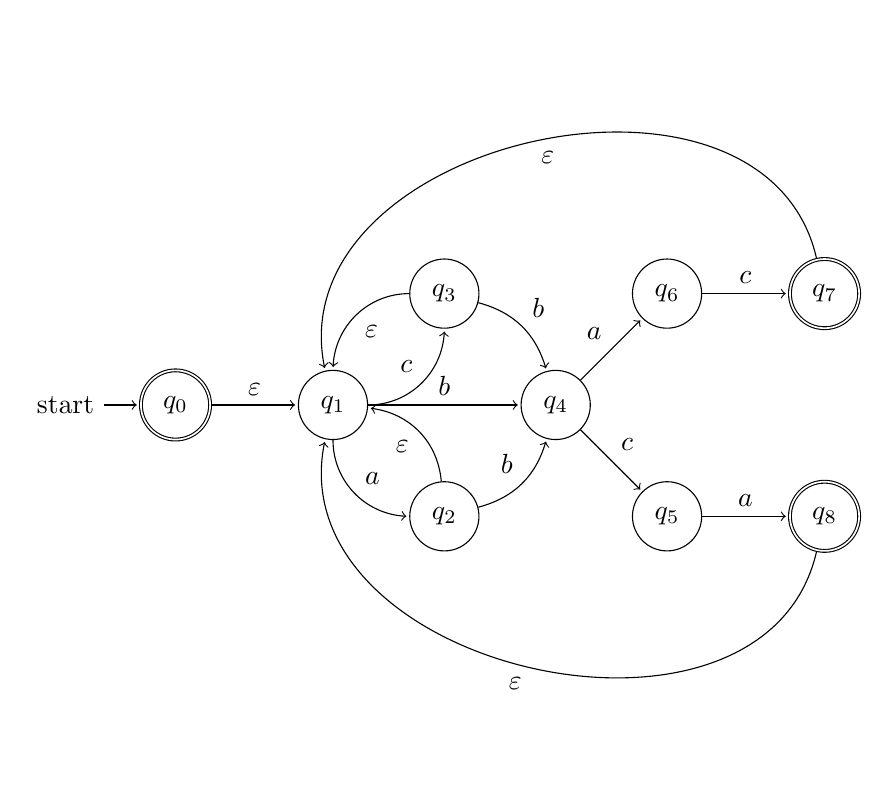
\begin{tikzpicture}[shorten >=1pt,node distance=2cm,on grid,auto]
        \node[state, initial, accepting]   (q0)                       {$q_0$};
        \node[state]   (q1) [right of=q0]                      {$q_1$};
        \node[state]   (q2) [below right of=q1]                       {$q_2$};
        \node[state]   (q3) [above right of=q1]                       {$q_3$};
        \node[state]   (q4) [above right of=q2]                       {$q_4$};
        \node[state]   (q5) [below right of=q4]                       {$q_5$};
        \node[state]   (q6) [above right of=q4]                       {$q_6$};
        \node[state, accepting]   (q7) [right of=q6]            {$q_7$};
        \node[state, accepting]   (q8) [right of=q5]            {$q_8$};


        \path[->]   (q0) edge node {$\epsilon$} (q1)
        (q1) edge [bend right=45] node {$c$} (q3)
        (q1) edge [bend right=45] node {$a$} (q2)
        (q1) edge node {$b$} (q4)

        (q2) edge [bend right=40] node {$\epsilon$} (q1)
        (q2) edge [bend right] node {$b$} (q4)

        (q3) edge [bend right=45] node {$\epsilon$} (q1)
        (q3) edge [bend left] node {$b$} (q4)

        (q4) edge node {$a$} (q6)
        (q4) edge node {$c$} (q5)

        (q6) edge node {$c$} (q7)

        (q5) edge node {$a$} (q8)

        (q7) edge [bend right=90, distance=3cm] node {$\epsilon$} (q1)
        (q8) edge [bend left=90, distance=3cm] node {$\epsilon$} (q1)
        ;
    \end{tikzpicture}
\end{question}

\begin{question}
    {3b}
    {
        (3 points) Give a regular expression representing the set of all binary strings that end with an odd number of 1's, i.e. 1, 101, 1101, 0101100111, etc.
    }
    $(\Sigma)^*(01)(11)^* \cup (1)(11)^*$
\end{question}

\begin{question}
    {4}
    {
        Let L be the set of strings over the alphabet $\{0, -\}$ of the form $0^{n_1}-0^{n_2}-0^{n_3}-...-0^{n_k}$ where $n_i \neq n_j$ for $i \neq j$. In other words, strings in $L$ are sequences of repeated 0's separated by $-$, where none of the subsequences within the same string have the same length. $0-0000-00$, $00-0$, $0$, and $0000000-000-0000-00$ are examples of strings in $L$, but $000-000$, $0-00-0$, etc. are not.

        Prove that $L$ is not regular using the pumping lemma.
    }
    Assume, for the sake of contradiction, that $L$ is regular. Let $p$ be the
    pumping length, and let $s = 0^{2p}-0^{2p+1}-\dots-0^{3p-1}-0^{3p} \in L$.
    Since $|s| > |p|$ of the pumping lemma we know that any $s \in L$ can
    be split up such that $s = xy^iz \in L$ for $i \geq 0$.

    Now, let $y = 0^i$ for $i \in [1, p]$ and note that $|y| > 0$. Then $y$ must be a zero since $|xy| \leq p$.
    We observe that
    \begin{equation*}
        xyyz = 0^{2p+i}-0^{2p+1}-\dots-0^{3p-1}-0^{3p}.
    \end{equation*}
    However, $2p+i$ is equal to one of the exponents for the other sequences of 0s
    (i.e. $2p + i = n$ for some $n \in \set{2p, 2p + 1,\dots,3p}$ since $i \geq 1$).
    This is a contradiction. Therefore, $L$ is not regular.

\end{question}

\end{document}